\section{Agent-MD Framework}

\subsection{Overall Architecture and Agent Roles}
In this work, Agent-MD combines two forms of agency with scientific computation tools and persistent campaign records. The reasoning agent handles tasks that require flexible interpretation, principally campaign construction and event-triggered review. The rule-based campaign agent operates the production campaign by reading the approved campaign specification and current campaign state, selecting and dispatching the next permitted action, invoking scientific tools, and updating the campaign records. The two agents therefore differ in how they select actions rather than in whether they participate in the workflow.

As shown in Figure~\ref{fig:agent_md_architecture}, campaign construction begins with scientific inputs supplied by the researcher, including the objective, ordered conditions or path, target observables, constraints, and available tools. The reasoning agent converts these inputs into proposed model or system choices, a campaign plan, execution rules, and acceptance rules. The researcher reviews and approves the proposal, producing an explicit campaign specification that can be inspected and executed by the production workflow.

Production is organized as a stateful simulation campaign. A molecular system denotes a distinct model or composition, whereas a simulation state denotes that system at one prescribed condition together with its current configuration, sampling progress, analysis status, completion status, and provenance. When a new system is started, the rule-based campaign agent invokes model-construction tools and prepares the initial inputs. When the campaign advances from state $k$ to state $k+1$, the agent inherits the accepted predecessor state and generates the inputs required for the next prescribed condition. New-system construction and state-to-state progression are therefore distinct workflow actions.

Within each simulation state, the rule-based campaign agent coordinates a run--analyze--decide cycle. After each simulation segment, automated routines analyze the outputs and the approved continuation and acceptance rules are applied. An unfinished state is continued from its current restart, an accepted state is archived together with its supporting records, and a state that cannot be safely resolved by the approved rules is routed to review. Completion of a simulation segment therefore does not by itself imply completion of the simulation state.

During event-triggered review, the reasoning agent receives a structured review event and evidence bundle and proposes a response or modification. The proposal is validated before it can affect the campaign, and human review is used when required. Validated actions return to the rule-based campaign agent, which resumes execution and records the resulting changes. Persistent campaign state and provenance connect all three parts of the architecture and preserve the information required to continue, reproduce, and audit the campaign.

\begin{figure}[t]
    \centering
    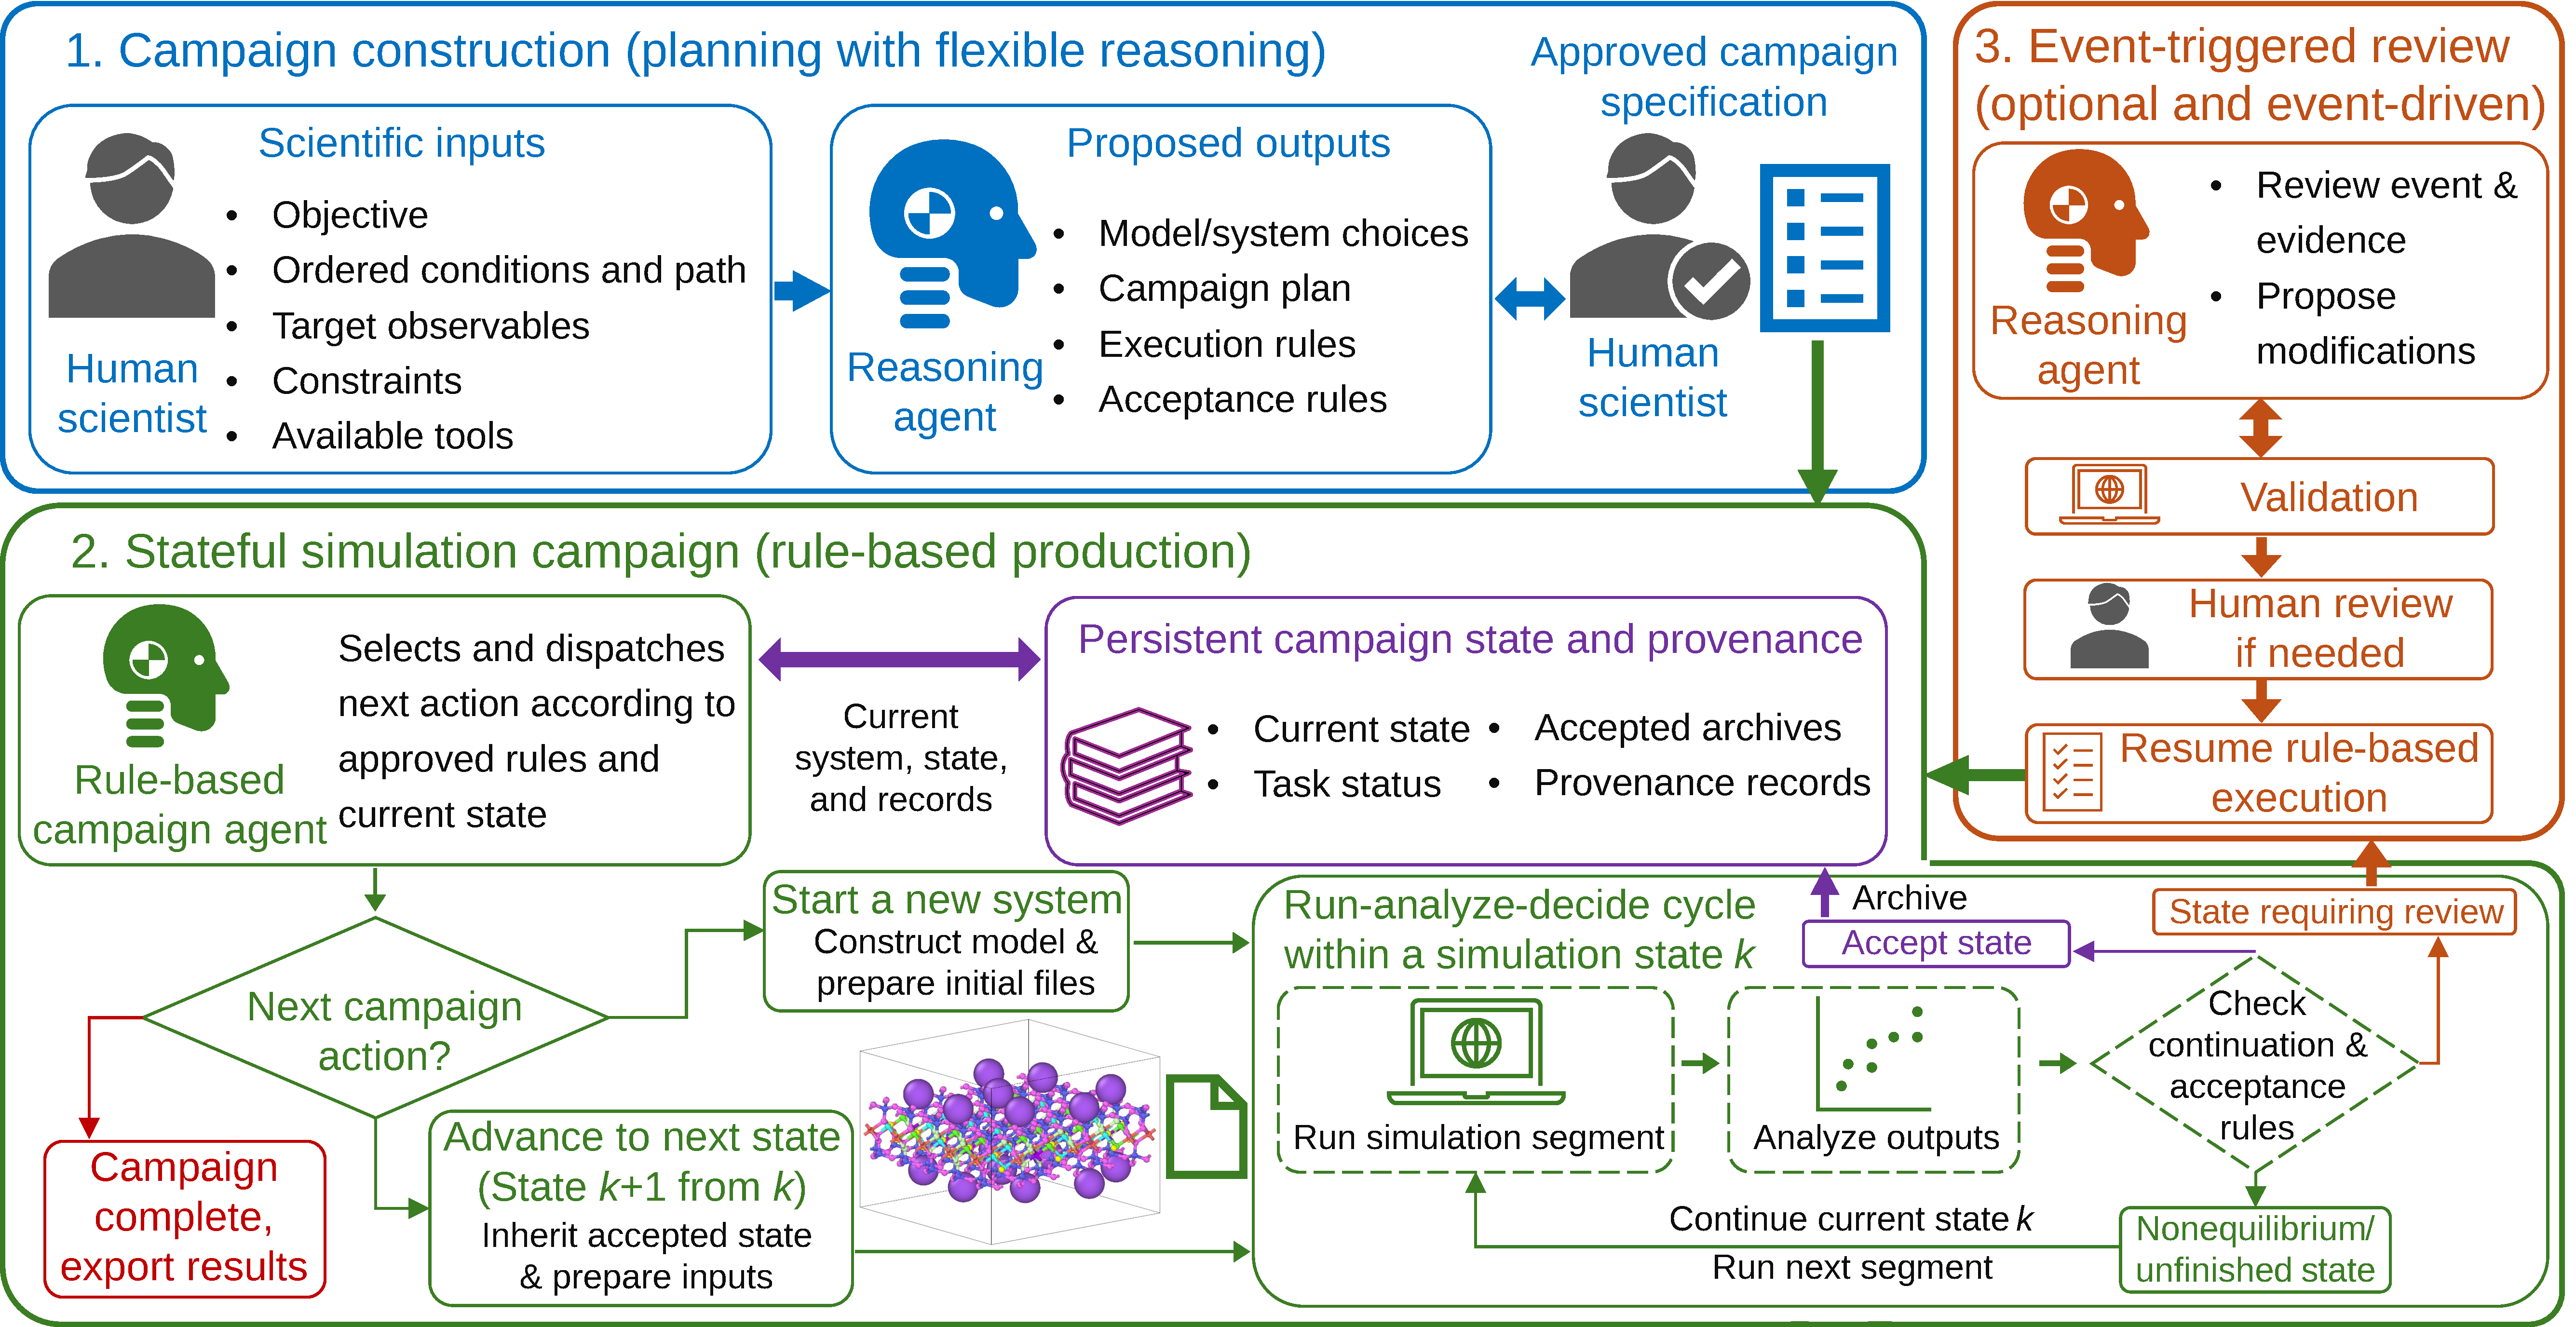
\includegraphics[width=0.98\linewidth]{../figures/fig1.pdf}
    \caption{Agent-MD architecture for stateful simulation campaigns.}
    \label{fig:agent_md_architecture}
\end{figure}

\subsection{Campaign Construction and System Preparation}

To demonstrate how the general Agent-MD framework is instantiated in a scientific workflow, we applied it to a montmorillonite water-vapor desorption campaign. The human scientist defined the scientific objective: follow the desorption pathway \(\mathrm{RH} = 0.9 \rightarrow 0.3 \rightarrow 0.1\), compare exchangeable-cation and layer-charge effects, and monitor total, interlayer, and external-surface water populations together with basal-spacing evolution. The objective specified the scientific comparison and observables, while the exact cation types, layer-charge levels, and resulting molecular models remained to be resolved during campaign planning.

The reasoning agent transformed this objective into a proposed campaign design specifying the molecular-system matrix, ordered RH-state sequence, target observables, execution rules, and acceptance rules. It proposed choices supported by the available preparation workflow rather than selecting every low-level simulation parameter. The human scientist reviewed and approved the proposal, producing the campaign specification used by the rule-based campaign agent; the reasoning agent neither approved the campaign independently nor directly ran the simulations.

Figure~\ref{fig:campaign_instantiation} presents this montmorillonite water-vapor desorption campaign as a concrete scientific instantiation of the general Agent-MD architecture in Figure~\ref{fig:agent_md_architecture}. It separates reasoning-agent campaign planning from preparation and stateful RH-dependent simulation by the rule-based campaign agent.

\begin{figure}[htbp]
    \centering
    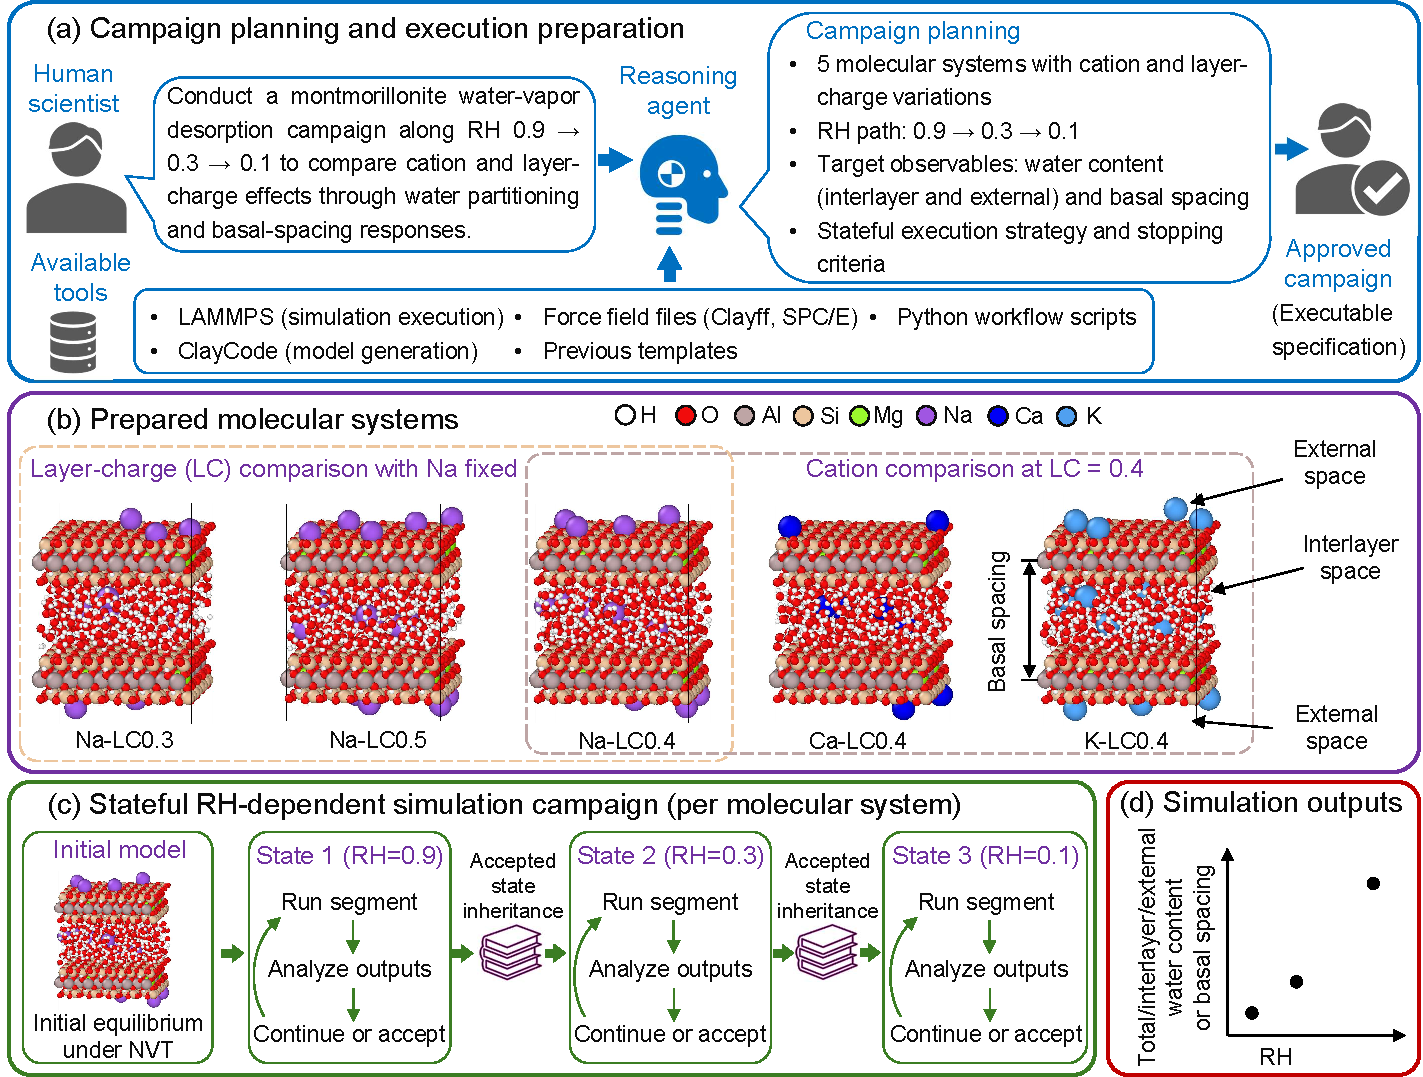
\includegraphics[width=0.98\linewidth]{../figures/fig2.pdf}
    \caption{Instantiation of Agent-MD for a montmorillonite water-vapor desorption campaign.}
    \label{fig:campaign_instantiation}
\end{figure}

The approved molecular-system matrix contained Na-LC0.4, K-LC0.4, and Ca-LC0.4 for the cation comparison and Na-LC0.3, Na-LC0.4, and Na-LC0.5 for the layer-charge comparison. Na-LC0.4 was shared between the two comparisons, giving five distinct molecular systems. Here, LC denotes the magnitude of the nominal negative layer charge, expressed in units of the elementary charge $e$ per $\mathrm{O}_{20}(\mathrm{OH})_{4}$ structural unit. Combining the five systems with the three researcher-prescribed RH states produced a planned stateful RH-dependent simulation campaign of 15 system--RH simulation states.

The approved campaign specification encoded the five-system matrix, prescribed RH sequence, target observables, continuation and acceptance policies, and state-transition rules. Five system-specific case records stored composition, charge, model size, and preparation parameters, while a machine-readable task plan represented dependencies among molecular-system preparation, equilibration, RH-specific production, analysis, archiving, and state progression. Together with the persistent campaign-state record, these files translated campaign planning into executable simulation tasks for the rule-based campaign agent.



The computational environment combined ClayCode for molecular-model generation, ClayFF force-field files and SPC/E water-model files for the molecular description, LAMMPS for GCMC--MD execution, Python workflow scripts for campaign control, and templates adapted from previously validated clay--water GCMC--MD protocols \cite{pollak2024claycode,cygan2004clayff,plimpton1995lammps,thompson2022lammps,wang2025ca}. After human approval, the rule-based campaign agent reads the campaign specification, invokes ClayCode to generate the prepared molecular systems, converts the resulting structure and topology files into LAMMPS-ready data files, and creates system- and state-specific inputs from the approved parameters and previous templates. The Python workflow then manages simulation launch and continuation, analysis, accepted state inheritance, archiving, and campaign-state updates. Automated validation checks verify expected cation counts, exchangeable-ion groups, ion placement partitions, molecule identifiers, atom types, charges, required files, and water-template compatibility before execution proceeds.

The prepared molecular systems, machine-readable specifications, initial state records, human-readable planning summaries, and preparation reports provide an auditable starting point for production. The rule-based campaign agent records the resulting system and state information in the persistent campaign state and provenance records. Agent-MD thus combines reasoning-agent campaign planning and human approval with rule-based campaign execution through established model-construction, simulation, and analysis tools. The corresponding campaign specifications, operational state records, final archive artifacts, figure-source data, and plotting scripts will be released at \url{GITHUB-URL}; the principal repository artifacts are summarized in Appendix~\ref{app:repo_artifacts}.

\subsection{Rule-Based Campaign Agent for Stateful Production}

The right panel of Figure~\ref{fig:campaign_instantiation} illustrates how each molecular system follows the prescribed RH path through a sequence of inherited simulation states. After campaign construction and system preparation, the rule-based campaign agent manages production over the approved system--state matrix. Each simulation state represents one molecular system at one prescribed RH condition together with its current configuration, sampling progress, analysis status, completion status, and provenance.

Production can enter the run--analyze--decide cycle in two ways. For a new molecular system, the rule-based campaign agent invokes the model-construction tools, prepares the initial files and inputs, records the system, and initializes its first prescribed simulation state. For a successor state, the agent selects the authoritative restart and relevant records from the accepted predecessor state, generates the next RH-specific input, and initializes state $k+1$ from state $k$. Constructing a molecular system and advancing that system along the ordered condition path are therefore distinct actions.

Within a simulation state, the rule-based campaign agent prepares the RH-specific GCMC--MD input, launches or resumes a LAMMPS segment through the scientific computation tools, and records the resulting monitor files, restart files, logs, and run-status records. Segmented execution is important because the required sampling effort is not known in advance and may differ substantially across molecular systems and RH conditions. Rather than requiring the researcher or reasoning agent to select the next action after every segment, the rule-based campaign agent selects actions from the approved rules, task dependencies, and recorded campaign state.

After each segment, automated analysis routines evaluate the monitored quantities used to judge completion. In the present GCMC--MD campaign, these include the total water population, interlayer and external-surface water populations, basal-spacing proxy, and basic simulation-health indicators. The analyzer computes final-window statistics and trend measures, and the rule-based campaign agent applies the configured continuation and acceptance rules. For an unfinished or nonequilibrated state, the agent generates the next segment from the current valid restart and continues the same run--analyze--decide loop. An unfinished state is not routed to review when the approved rules determine a safe continuation.

When a simulation state is accepted, the rule-based campaign agent selects and archives the authoritative restart, copies the supporting monitor and analysis records, updates persistent campaign state and provenance, and makes the accepted state available for state inheritance. The archive records include the system identity, RH value, final absolute timestep, selected restart path, convergence status, and supporting source files. A successor state is initialized from the accepted predecessor state rather than from an arbitrary latest file in a working directory, preventing downstream states from silently depending on stale, incomplete, or superseded outputs. When a state cannot be safely resolved by the approved rules, the campaign agent creates a review event and evidence bundle and routes the state to the review process described in Section~2.4.

A further requirement in sequential RH campaigns is to distinguish the absolute timestep inherited through LAMMPS restarts from the sampling performed within the current simulation state. Because successor states are initialized from accepted predecessor restarts, their absolute timesteps may begin far from zero. Agent-MD therefore records both the absolute simulation timestep and RH-local elapsed steps. Production budgets and continuation limits are applied to RH-local sampling effort, while the absolute timestep is retained for restart consistency and provenance. This distinction allows acceptance to be evaluated relative to the current simulation state at its prescribed RH condition rather than the cumulative history of the trajectory.

\subsection{Event-Triggered Review and Decision Validation}

Routine production does not require invocation of the reasoning agent because it is operated by the rule-based campaign agent. During normal production, the campaign agent launches or resumes simulations, selects restarts, initiates convergence analysis, continues unfinished states, archives accepted states, and advances along the prescribed RH path according to approved rules. Review is triggered only when the campaign agent reaches a production state that cannot be safely resolved as another permitted action using those rules.

Event-triggered review is activated after a workflow action completes or fails, rather than by continuous model polling. The rule-based campaign agent examines the structured action result, stop reason, and recorded workflow context. If the outcome cannot be safely handled by approved rules, the campaign agent creates a review event and gathers the associated evidence bundle for reasoning-agent or human review.

The current implementation defines five review-event identifiers: \texttt{CONVERGENCE\_ANOMALY},\linebreak \texttt{PROVENANCE\_CONFLICT}, \texttt{UNKNOWN\_FAILURE},\linebreak \texttt{NEEDS\_REASONING}, and \texttt{BATCH\_COMPLETE}. They represent anomalous convergence behavior, inconsistent provenance, an unclassified execution failure, a state requiring flexible interpretation, and a completed batch requiring additional review, respectively. These identifiers are implementation-level labels rather than a universal taxonomy. Routine successful completion, safe continuation, and archiving do not themselves require reasoning-agent review; \texttt{BATCH\_COMPLETE} is relevant only when completion still requires additional review.

For each review event, the rule-based campaign agent constructs a compact evidence bundle from persistent campaign state and provenance records and associated artifacts. The evidence may include action status, stop reason, system identity, RH condition, analysis summaries, campaign-agent decisions, archive metadata, restart provenance, monitor-file summaries, error signatures, and relevant status records. The workflow packages the review event and evidence as a focused task for the reasoning agent. The same bundle can be inspected by a human reviewer, making the review interface auditable even when the reasoning agent is not invoked.

In the present implementation, the optional reasoning agent was implemented through the Codex CLI and powered by GPT-5.5. When invoked, the Codex CLI reasoning agent receives a structured event record and evidence bundle and returns a schema-constrained JSON recommendation. Runtime invocation is disabled by default and can occur only when event-triggered review is enabled, an eligible event has been emitted, and the guarded invocation policy permits the call. The corresponding machine-readable inputs and output are stored as \path{agent_event.json}, \path{evidence_bundle.json}, and \path{agent_decision.json}, respectively.

The reasoning agent proposes a response or modification but does not directly edit the simulation or launch jobs. The proposal must pass schema, policy, and applicable workflow validation before it can affect production. Permitted validated outcomes include acknowledging the event, continuing rule-based execution, retrying a safe action, stopping the campaign, or recording a requirement for human review. Human review is used when the proposal remains unresolved, exceeds permitted actions, or otherwise requires scientific approval; it is not mandatory for every review event. Invalid, missing, stale, or failed recommendations fall back to a conservative review-required state. Additional safeguards include duplicate-fingerprint blocking, call caps, recursion guards, and restrictions on accepted actions or parameter changes.

A validated response is returned to the rule-based campaign agent, which resumes, stops, retries, or records a human-review requirement according to that response and updates the campaign records. Review is tied to recorded workflow state, not to elapsed wall time, simulation length, or routine task completion. This protocol allows the reasoning agent to propose a response without transferring direct simulation control and preserves a validated return path to persistent production.
